\chapter{Experiment}

In this chapter we will discuss the simulations, the gathered data as well as the results. We will divide the chapter into three parts. In the first one we will make changes in the demand side of the model, in the second part we will alter the supply side and lastly we will compare the results and discuss about the results.

As previously mentioned in the past chapter we implemented category C1 and C2. Thus we will divide the supply section into two parts. The first one will contain the simulations of C1 and the second one of C2. We will alter the variables of the mentioned categories one at a time, leaving the rest of the variables untouched. 

Before we can start simulating we have to empirically search for minimum number of iteration that the model has to make in order for the market (ratios and KPIs) to converge. We will set the expLength (in second main loop) to a large number an plot it until we achieve a minimum number. As shown in the figure bellow, with static variables, the smallest value for expLength is 1500 in order to be completely sure that it will converge for all other $\lambda$ and probabilities to be tested. Then we will run the plots over the variable that will be tested as x-axis and not time/iterations.

\begin{figure}
    \centering
    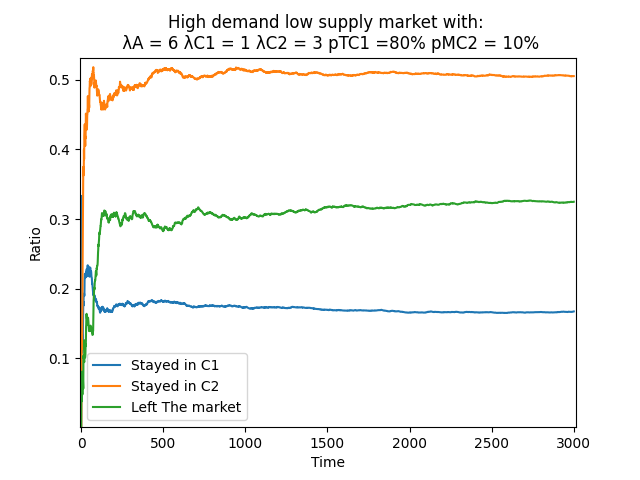
\includegraphics[width=0.6\linewidth]{figures/Rates_of_total_agents_distribution_over_time.png}
    \caption{Example of a market simulation with fixed variables over 3000 iterations with high demand and low supply converging.}
    \label{fig:convergence}
\end{figure}


\section{Changes in Demand}

In the demand side of the market there is one variables that can be changed. This variable being $\lambda$\A or the rate at which agents arrive to the market. In the next sections we will present market data while subject to changes in $\lambda$A.

\subsection{Simulations}

We will simulated the market with a wide range of values for $\lambda$A (0 to 20), going from a high supply and low demand in the early stages of the simulation and ending with very high demand and low supply. This with the purpose of demonstrating a shift of the market towards high demand and low supply Bellow we can find the data from the simulation for such a scenario. There is a graph for the mentioned KPIs as well as one for the average waiting times. For the extended results please refer to appendix \ref{fig:lATable} 


\begin{figure}
    \centering
    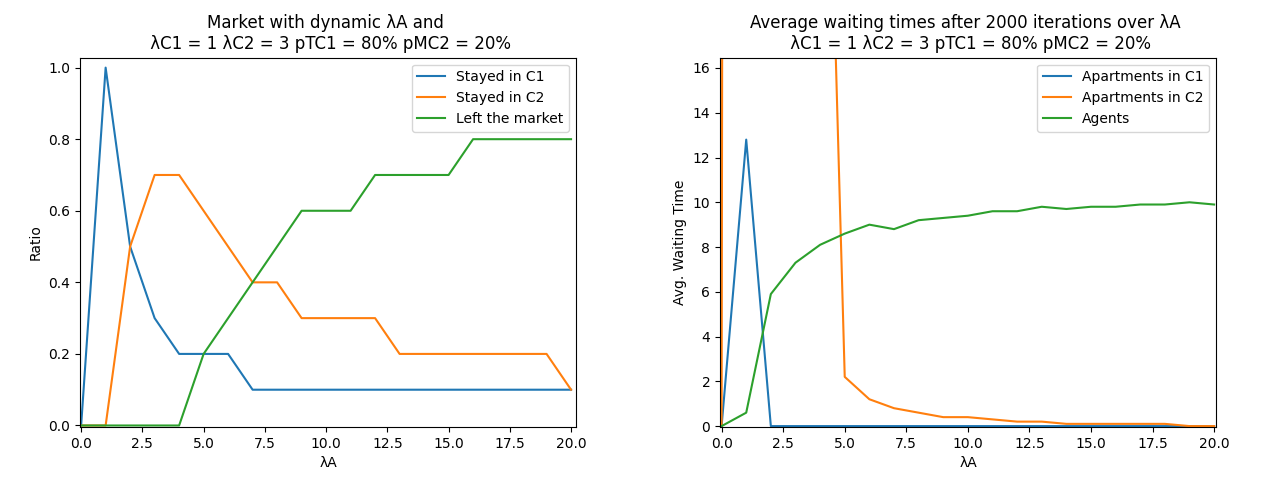
\includegraphics[width=1\linewidth, height = 7cm]{figures/lambdaA.png}
    \caption{Left: KPIs for changes in $\lambda$A. Right: Average waiting times of apartments in C1, C2 and the agents over changes in $\lambda$A.}
    \label{fig:KPIslambdaA}
\end{figure}

\subsection{Observations}

From \ref{fig:KPIslambdaA} we can see that the ratio of agents that left the market grow towards 1 and the ratio of agents that found some kind of accommodation (either in C1 or C2) falls towards 0. This is very straight forward since the supply never grows but the demand grows at a constant rate. At some point almost 100\% of the agents that arrive will not have the chance of finding accommodation an leave the market. Therefore we can assume that by running $\lambda$A towards infinity the ratio of agents that left/found will converge against 0 or 1 respectively.

The average waiting times from \ref{fig:KPIslambdaA} demonstrates that the more agents arrive to the market the higher the waiting time to find accommodation it gets. It eventually converges against 10, which is the average maximum waiting time assigned to them via the exponential distribution. This means they will eventually wait all the time then have since there is no accommodation possible and will leave the market. From the other side, the apartments waiting times converge against zero, since there is a point with too much demand but the demand stays constant. We can also observe that the waiting time of the houses starts at a high average and ends with zero. This is because in the beginning there are not enough agents to take all houses and thus are never occupied. We can also see that the spike in C1 is considerably smaller and falls at a faster rate than the one in C2. This is because agents prefer the C1 for its higher utility than C2.

We can see from these two figures that there is an equilibrium in the market. This is point is reached, when the sum of the agents equals the sum of apartments. In this precise example when $\lambda$A is equal to four. Here the ratio at which new apartments arrive to the market is the same as the ratio at which agents arrive. We can use this equilibrium to model the desired market. In this case we simulate with focus in a market with $\lambda A \geq 4$. 


\section{Changes in Supply}

The supply side of the model offers a wider variety of variables to manipulate. As mentioned we divided the next section into changes in C1 and C2. In category 1 we can change $\lambda$C1 that regulate the arrival of the new apartments to the market in C1 as well as \textbf{pTC1} that depicts the probability of the agent to take a matched accommodation in C1. For category 2 we can alter the variable $\lambda$C2 that is analogous to the one in category C1 and \textbf{pMC2} that computes the probability of the agent of being matched to an apartment. Note that in C1 there is no patching probability since it depends on the FCFS queue and in C2 there is no taking probability yet since C3 isn't implemented and there is no real decision to be made here.

\subsection{Changes in C1}

In this section we will present simulations of the market by changing the values $\lambda$C1 and \textbf{pTC1} but leaving the rest static. We will be altering the supply of apartments in C1 while leaving the arrivals of agents in the market and apartments in C2 constant.

\subsubsection{Simulations}

We ran the first simulation over $\lambda$C1 from 0 to 20 and plotted first over the KPIs ans then over the average waiting times. The table with the raw data for these plots can be found in the appendices of this paper. 

\begin{figure}
    \centering
    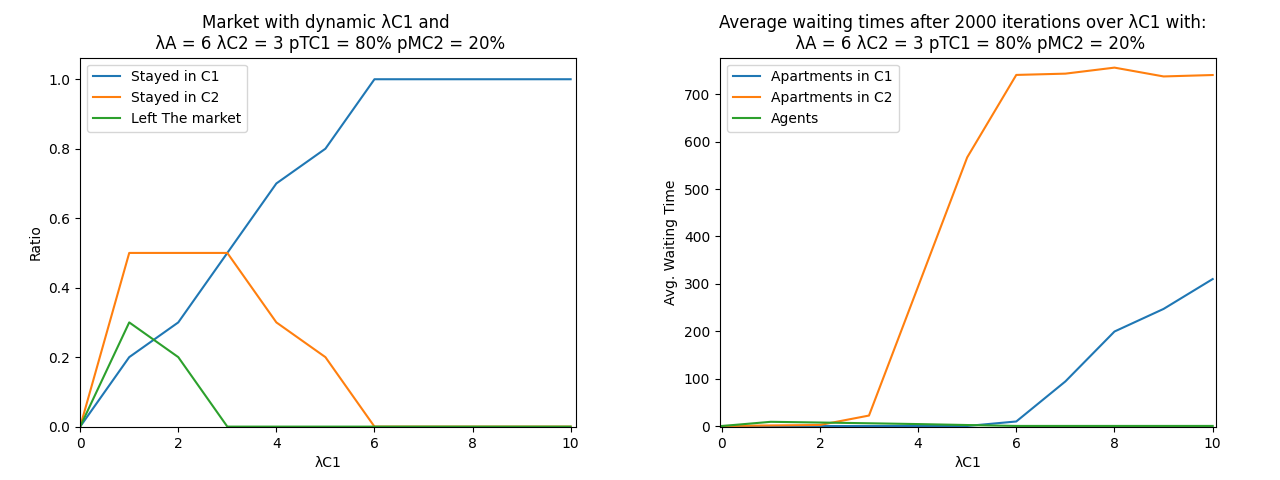
\includegraphics[width=1\linewidth, height = 7cm]{figures/lambdaC1inC1.png}
    \caption{Left: KPIs for changes in $\lambda$C1. Right: Average waiting times of apartments in C1, C2 and the agents over changes in $\lambda$C1.}
    \label{fig:c1lambdac1}
\end{figure}

Then we ran a second simulation with \textbf{pTC1} from 0 to 10 and changed the static variables since the effect of \textbf{pTC1} over C1 is better seen in a market with a more balanced demand-supply chain. We also made the intervals between data points smaller. They were increased by 0.5 instead of 1. This way we can simulate a short interval with more detail. To see the extended results please refer to \ref{fig:l1c1table} and \ref{fig:ptc1table}

\begin{figure}
    \centering
    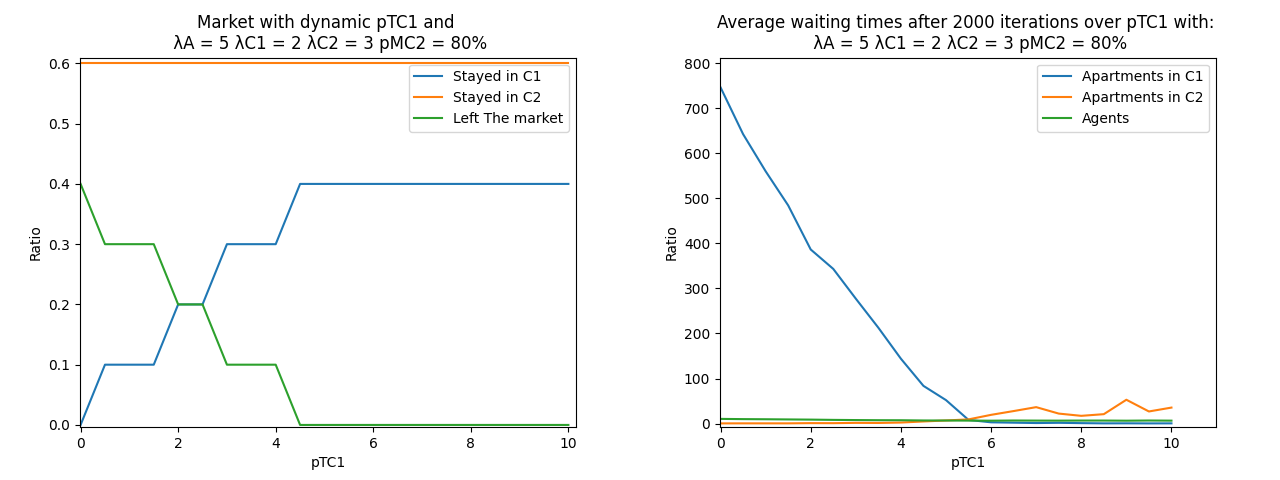
\includegraphics[width=1\linewidth, height = 7cm]{figures/pTC1.png}
    \caption{Left: KPIs for changes in \textbf{pTC1}. Right: Average waiting times of apartments in C1, C2 and the agents over changes in \textbf{pTC1}.}
    \label{fig:pTC1}
\end{figure}

\subsubsection{Observations}

From the simulations over $\lambda$C1 in figure \ref{fig:c1lambdac1} we can clearly observe, that the agents will always prefer C1 over C2. We can see that from interval 1 to 3 C2 has reaches its maximum since it is covering the supply in the market by its own with little apartments in C1. When  $\lambda$C1 takes the value of 3 the market hits its equilibrium point and C1 and C3 are equal. Here it is also important to remark, that from this point onwards no more agents have the necessity to leave the market. Afterwards C1 keeps taking demand away from C2 until all apartments in C2 are empty and all apartments from C1 are taken. Another example is how after the equilibrium point, the waiting times of C2 increase constantly while waiting times of C1 stay at zero just until the supply is greater than the demand when $\lambda$C1 is equal to 6.

Moreover we observed that for very low \textbf{pTC1} the waiting times of C1 increases considerably \ref{fig:pTC1}. However if we let this variable run we can see that the average waiting time of C1 rapidly decreases and when it hits 6\% it is already close to zero. This is because even though the probability of taking the apartment is very low, the agents will still prioritize accommodation in C1 and will wait in the FCFS queue again. Furthermore we can see how the lower the probability it is the more agents leave the market until it is around 6\% then the market converges, 60\% of the agents stays in C2 and 40\% in C1.

\subsection{Changes in C2}

In this section we will observe the market by changing the variables that control the supply side of the market specifically them of C2. The variables at our reach for this simulations are $\lambda$C2 and \textbf{pMC2}. 

\subsubsection{Simulations}

In figure \ref{fig:lambdac2} we simulated over $\lambda$C2 with an interval from 0 to 6. We chose a small interval for This since the plot converged quickly. We left the rest of the variables fixed as in the previous simulations of C1 and Demand. For the average waiting times plot we cut the plot when $\lambda$C2 reached 4. This choice was made since the waiting time of the apartments in C2 grew quickly and eventually the line for agents would disappear from the visual field.

\begin{figure}
    \centering
    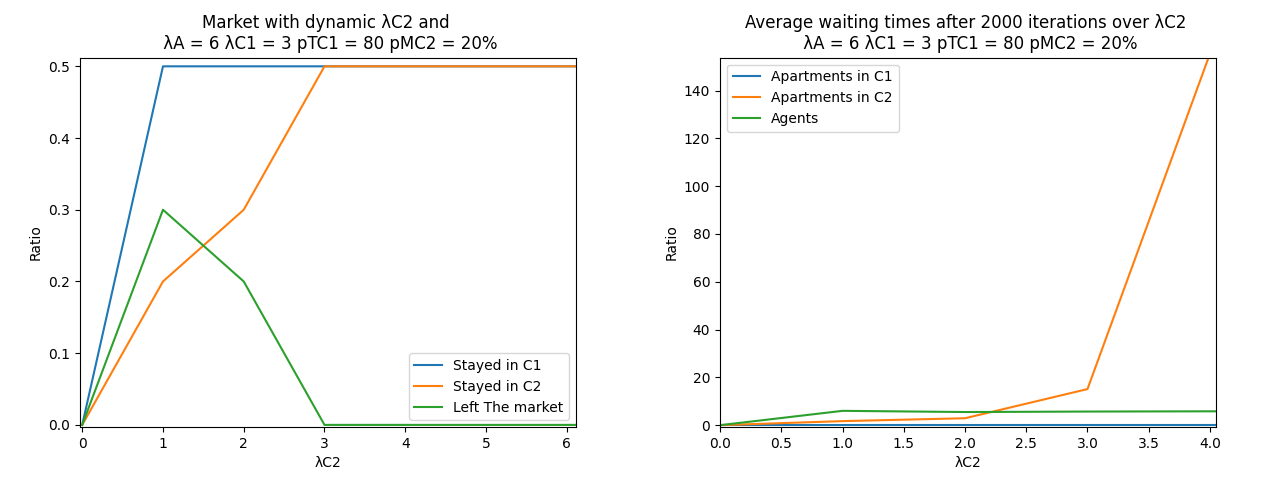
\includegraphics[width=1\linewidth, height = 7cm]{figures/lambdaC2.png}
    \caption{Left: KPIs for changes in $\lambda$C2. Right: Average waiting times of apartments in C1, C2 and the agents over changes in $\lambda$C2.}
    \label{fig:lambdac2}
\end{figure}

Then we plotted over the matching probability \textbf{pMC2} from 0 to 40. For this simulation we chose smaller lambdas since the simulation running time was very high and this shortened the running time considerably. Moreover with these new values for the fixed variables the effects of \textbf{pCM2} on the market are more pronounced. The extended results can be found in \ref{fig:lc2table} and \ref{fig:pmc2table}

\begin{figure}
    \centering
    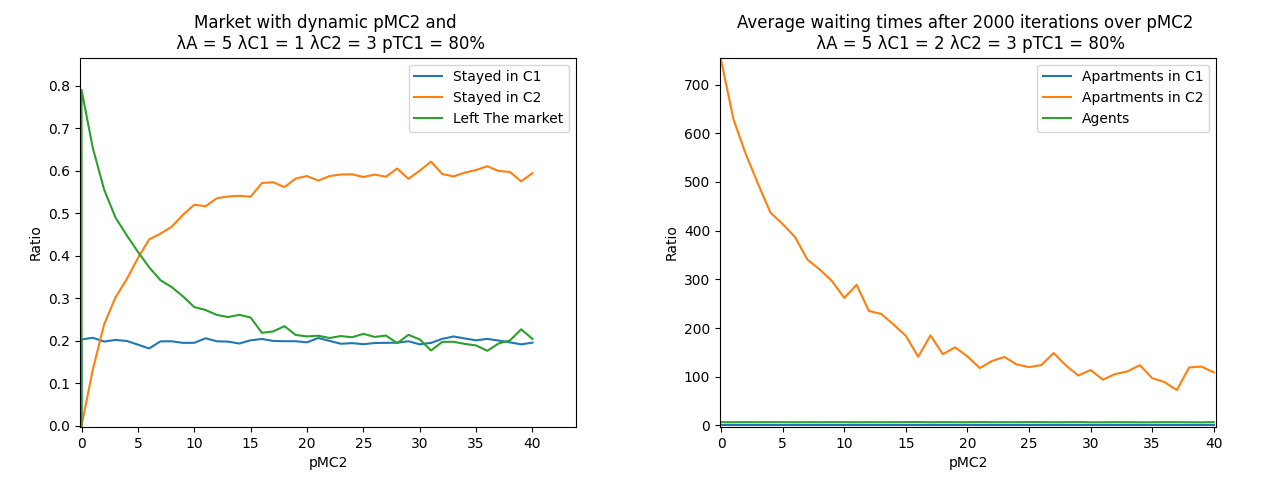
\includegraphics[width=1\linewidth, height = 7cm]{figures/pMC2.png}
    \caption{Left: KPIs for changes in \textbf{pMC2}. Right: Average waiting times of apartments in C1, C2 and the agents over changes in \textbf{pMC2}.}
    \label{fig:pMC2}
\end{figure}

\subsubsection{Observations}

From figure \ref{fig:lambdac2} we can observe, that over the whole period of time, the Houses in C1 where occupied, including when there were an over supply of accommodations in C2. Moreover the equilibrium point here is reached when $\lambda$C2 is equal to 3. At this point supply and demand are equal and the market is balances. Afterwards there are zero or close to zero agents leaving the market. For an agent to leave the market under these circumstances he would need to have spawned with a very low maximum time in order to not have had a chance in the FCFS queue and little time to be matched to apartments int C2. Furthermore, from the average waiting times we can see, that from the point where the market hits its equilibrium, any extra apartment in C2 will not be occupied and the waiting times will rise. We can also see that from  interval 2 to 3 the average waiting time of C2 is rising but not at the same rate after point 3. This is because even though there are more than enough houses to accommodate the whole demand of the market, the against will still prefer to wait for accommodation in C1 and waiting until the last opportunity to take something in C2.

Additionally we can see from figure \ref{fig:pMC2}, that in a balanced market (or a market in equilibrium) where demand equals the supply, if the matching probability for C2 is too low, many agents will not be able to find any accommodation. Moreover we can see that after crossing a probability of 30\% the market no longer reacts to this probability and it converges. This plot also relates directly to the average waiting times of the apartments in C2, where after the probability is 30\% the waiting time doesn't change much. On the other hand any matching probability lower than 30\% results in a higher waiting time of the houses in order to find an agent to accommodate. In order to see all the data please refer to the appendices of this paper where the data for all plots will be presented.

\section{Overall Data Analysis}

On this section we will discuss the results of the simulations presented in the section above. We will interpret and discuss the results. From the early observations we can see, that the market hits equilibrium points where the demand and supply can support each other. Moreover we saw that for an equilibrium point where the agents don't leave the market. The supply side hast to be lightly higher than the demand side when the taking and matching probability are low, thus leaving some apartments empty. On the other hand in order to have an equilibrium where all houses are taken and the supply and demand are exactly equal to each other, the take and match probability should be as close as possible to 100\%. This is an interesting phenomena and the explanation for that is that since the market is over saturated from the demand side, no matter if the probability is low since there are so many agents awaiting for accommodation that eventually one of them will take the place. Examples of these probabilities having to be very low in order to have an effect on the market are \ref{fig:pTC1} and \ref{fig:pMC2}. A big effect this probabilities are the waiting times, we observed that the lower the probability the higher the waiting times. This is because the agents have a smaller chance of taking\/matching to a certain apartment and if not they will wait more or go to the back of the FCFS queue.

Furthermore we saw that agents have strong preferences towards accommodations that offer a higher utility and they would even risk to have to leave the market in order to find accommodation in the public subsidised sector. We observed, that if it where possible the whole population of agents would stay in C1 replacing C2 entirely and at some point is no longer profitable to add more apartments in C2 since they will not be used. Figure \ref{fig:c1lambdac1} is a good example of that, as well as \ref{fig:lambdac2}.


Lastly we saw that we could divide all plots into three intervals and categorise them. From the supply side of the market, first we have the early stages of the plot where there is not enough apartments for the market and we observed agents leaving the market. Then we have a point where the market reaches its equilibrium and at the end leaving the variables to "infinity" the market converges (with all agents having accommodation) and the average waiting times of the apartments with low utility sky rockets. On the other hand the simulations of the demand side of the market can also be always divided into three parts. Firstly there are not enough agents to fulfill the needs of the supply side of the market, the waiting times of the apartments are very high and those of the agents very low. Then the equilibrium point is reached as in the simulations for the supply side and all agents are accommodated. Lastly the by letting the agents in the market converge against infinity we will see that almost all agents will leave the market and their waiting times rises, on the other hand all possible accommodations in C1 and C2 are met and the ratio of arrived agents to taken accommodation will converge to zero. On the next section we will discuss about the possible application this software could have and how could it be improved and expanded

